\documentclass{beamer}

\usepackage[francais]{babel}
\usepackage[utf8]{inputenc}
\usepackage[T1]{fontenc}
\usepackage{graphicx}
\usepackage{graphics}
\usepackage{color}
\usepackage{textcomp}
\usepackage{pifont}
\usepackage[normalem]{ulem}
\usepackage{times}
\usepackage{hyperref}
\usepackage{verbatim}
\usepackage{amsmath}
\usepackage{amsthm}
\usepackage{amsfonts}
\usepackage[mathscr]{euscript}
\usepackage{pgfpages}
\usepackage{listings}
\usepackage{subfigure}
\usepackage{algorithm}
\usepackage[noend]{algorithmic}
\usepackage{pdftricks}
\usepackage{mathrsfs}
\usepackage{array}
\usepackage{fancybox}
% \usepackage{columns}
\usepackage{multirow}
\usepackage{url}
\usepackage{tikz}
\usepackage{colortbl}
%\usepackage{cite} %DO NOT FUCKING USE CITE ON BEAMER !!! LOST 30 GODDAM' MINUTES ON THIS SHIT !!!
\usepackage{mathabx}
\usepackage{amssymb}
\usepackage{eurosym}
\usepackage{wasysym} % ch0

\let\texteuro\euro

\hypersetup{colorlinks,%
            citecolor=black,%
            filecolor=black,%
            linkcolor=black,%
            urlcolor=blue}

%\addtolength{\parskip}{10pt}

\usetikzlibrary{calc}

\mode<presentation>
\setbeamertemplate{footline}[frame number]
\setbeamercovered{transparent}
\usetheme[navigation]{ESI}

%lst
\definecolor{comment-green}{RGB}{0,166,80}
\lstset{language=C++,
  keywordstyle=\lst@ifdisplaystyle\bf\fi\color{blue!60},
  commentstyle=\color{comment-green},
  stringstyle=\color{red},
  basicstyle=\lst@ifdisplaystyle\tiny\else\tt\fi,
  morekeywords={
    constexpr,concept,decltype,nullptr,nullptr_t,noexcept,final,override},
  frame=single,
  xleftmargin=0.5cm,
  numbers=left,
  tabsize=2}

%title
\subtitle{Langage \texttt{C} / \cpp}
\author{R. Absil}
\date{\today}

%styles
\theoremstyle{definition}
\newtheorem{thm}{Théorème}
\newtheorem{conj}[thm]{Conjecture}
\newtheorem{deff}[thm]{Définition}
\newtheorem{prop}[thm]{Propriété}
\newtheorem{lem}[thm]{Lemme}
\newtheorem*{lem*}{Lemme}
\newtheorem{cor}[thm]{Corollaire}
%\newtheorem{example}{Exemple}
\newtheorem{remark}{Remarque}
\newtheorem{exo}{Exercice}

%typeset
\newcommand{\ie}{{\emph{i.e., }}}
\newcommand{\eg}{{\emph{e.g., }}}
\newcommand{\etal}{{\emph{et al.}}}
\newcommand{\rrceil}{\unichar{"2308}}
\newcommand{\sloand}[2]{\footnote{N. J. A. Sloane - OEIS Foundation - \texttt{www.oeis.org}, Sequence #1 - #2.}}

%math
\newcommand{\IN}{{\mathbb N}}
\newcommand{\IQ}{{\mathbb Q}}
\newcommand{\IR}{{\mathbb R}}
\newcommand{\IZ}{{\mathbb Z}}
\newcommand{\IP}{{\mathbb P}}
\newcommand{\IC}{{\mathbb C}}
\newcommand{\bigo}{{\mathcal{O}}}
\renewcommand{\mod}{\bmod}
\newcommand{\ssi}{\Leftrightarrow}
\newcommand{\then}{\Rightarrow}
\newcommand{\fle}[1]{\stackrel{#1}{\longrightarrow}}
\newcommand{\suchthat}{~\big|~}
\newcommand{\floor}[1]{\left\lfloor #1 \right\rfloor}
\newcommand{\ceil}[1]{\left\lceil #1 \right\rceil}
\DeclareMathOperator*{\argmin}{argmin}
\DeclareMathOperator*{\argmax}{argmax}

%tikz
\tikzstyle{_vertex}=[fill=white, circle,minimum size=12pt,inner sep=1pt]
\tikzstyle{_blackv}=[fill=black, circle,minimum size=8pt,inner sep=1pt]
\tikzstyle{_dot}=[fill=black, circle, minimum size = 1mm, inner sep=0pt]
\tikzstyle{_bigvertex}=[fill=white, circle,minimum size=21pt,inner sep=1pt]
\tikzstyle{_arc}=[->, >=stealth]
\tikzstyle{_boldarc}=[->, >=stealth, line width=2pt]

\newcommand{\cpp}{\texttt{C++}}
\newcommand{\java}{\texttt{Java}}


\title{Ch. 3 - Fonctions}

\begin{document}
\begin{frame}
  \titlepage
\end{frame}

\begin{frame}
  \frametitle{Table des matières}
  \footnotesize \tableofcontents[pausesections,pausesubsections]
\end{frame}


\section{Introduction}

\begin{frame}
\frametitle{Utilité}
\begin{itemize}[<+->]
\item «~Ensemble d'instructions qui effectue une tâche~»
\item Peut être \emph{appelé} au sein d'un programme
\end{itemize}
\begin{exampleblock}<+->{Avantages}
	\begin{itemize}[<+->]
	\item Permet de découper le travail en parties indépendantes
	\item Permet de réutiliser du code
	\item Limite la redondance
		\begin{itemize}
		\item Moins de « copier / coller »
		\item Maintenabilité augmentée
		\end{itemize}
	\item Augmente la lisibilité
	\end{itemize}
\end{exampleblock}
\end{frame}

\begin{frame}
\frametitle{Caractéristiques}
\begin{enumerate}[<+->]
\item Possède des paramètres et un retour
	\begin{itemize}
	\item \texttt{sqrt} prend en paramètre un flottant et retourne un flottant
	\end{itemize}
\item En \texttt{C}, identifiées par leur nom uniquement
	\begin{itemize}
	\item Pas de surdéfinition possible
	\end{itemize}
\item En \texttt{C}, toutes les fonctions sont dites «~indépendantes~»
	\begin{itemize}
	\item Déclarées en dehors de toute classe
	\end{itemize}
\item Plus qu'une fonction mathématique
	\begin{itemize}
	\item Effectue un travail
	\item Possibilité de modifier les paramètres
	\item Peut ne rien retourner (\lstinline|void|)
	\end{itemize}
\end{enumerate}
\end{frame}

\begin{frame}[containsverbatim]
\frametitle{Illustration}
\begin{itemize}
\item Fichier \texttt{surdef.c}
\end{itemize}
\begin{lstlisting}
int f(int i)
{
	printf("Integer %d\n", i);
	return 0;
}

int f(double d) //you can't overload
{
	printf("Double %f\n", d);
	return 0;
}

int f(int i, int j) //you still can't, even with more params
{
    printf("Integers %d and %d\n", i, j);
    return 0;
}
\end{lstlisting}
\end{frame}

\begin{frame}
\frametitle{Déclaration et définition}
\begin{itemize}
\onslide<1-> \item Toute fonction doit être déclarée et définie
	\begin{itemize}
	\onslide<2->\item Possibilité de séparer la déclaration de la définition
	\onslide<3->\item Parfois nécessaire
	\end{itemize}
\end{itemize}
\begin{center}
\visible<4-|handout:1>{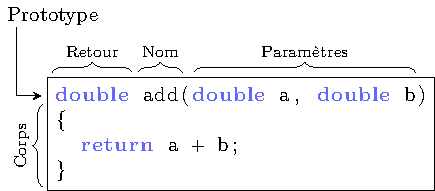
\includegraphics[width=.7\textwidth]{pics/fct.pdf}}
\end{center}
\begin{itemize}
\onslide<5-> \item Seul les types des paramètres sont nécessaires dans le prototype
\onslide<6-> \item Pour rappel, les fonctions \emph{doivent} être déclarées avant d'être utilisées
\onslide<7-> \item Déclaration possible au sein d'un bloc
\end{itemize}
\end{frame}

\begin{frame}[containsverbatim]
\frametitle{Exemple}
\begin{itemize}
\item Fichier \texttt{before.c}
\end{itemize}
\begin{lstlisting}
int main()
{
	print("Hello");
}

void print(const char* s)
{
	printf("%s\n", s);
}
\end{lstlisting}
\begin{itemize}
\item Déclaration anticipée
\end{itemize}
\begin{lstlisting}
void print(const char*);

int main()
{
	print("Hello");
}

void print(const char* s)
{
	printf("%s\n", s);
}
\end{lstlisting}
\begin{itemize}
\item Même principe en \cpp
\end{itemize}
\end{frame}

\begin{frame}[containsverbatim]
\frametitle{Les fonctions sans arguments}
\begin{itemize}
\item En \texttt{C} uniquement, si on veut qu'une fonction n'accepte aucun argument, il faut écrire \lstinline|void| dans la liste des paramètres
\item Si on déclare \lstinline|void f();|, la fonction \texttt{f} accepte un nombre arbitraire d'arguments (et les ignore)
\end{itemize}
\begin{lstlisting}
void f() {}
void g(void) {}

int main()
{
    f();
    f(1); //ok
    f(1,2); //ok
    
    g();
    //g(1); //ko    
}
\end{lstlisting}
\end{frame}

\section{Passage d'argument}

\begin{frame}
\frametitle{Passage par valeur}
\begin{itemize}[<+->]
\item Par défaut, à chaque appel d'une fonction, une \emph{copie} des paramètres est envoyée à la fonction
	\begin{itemize}
	\item Dans le cas d'un type de base, on copie la valeur
	\item Dans le cas d'une \lstinline|struct| (\texttt{C}), on copie les attributs
	\item Dans le cas d'un objet (\cpp), on appelle le constructeur de recopie (cf. Ch. ?)
	\end{itemize}
\item «~Ne permet pas~» de modifier les paramètres
\item La valeur de retour est également transmise par valeur	
\end{itemize}
\begin{exampleblock}<+->{Avantages}
	\begin{itemize}[<+->]
	\item Pas d'effet de bord
	\end{itemize}
\end{exampleblock}
\begin{alertblock}<+->{Inconvénients}
	\begin{itemize}[<+->]
	\item Performances réduites
	\end{itemize}
\end{alertblock}
\end{frame}

\begin{frame}
\frametitle{Mécanisme}
\begin{center}
\begin{tikzpicture}
\node[draw] at (0,0) 
{
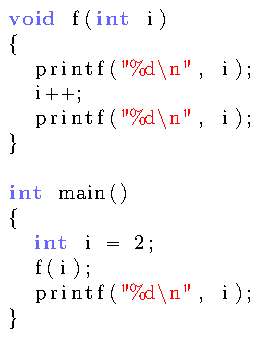
\includegraphics[width=4cm]{pics/sample-value.pdf}
};

\node at (7.5,3.5) {Pile};
\draw (6,-3) -- (6,3);
\draw (9,-3) -- (9,3);

%\foreach \i in {-2.5,-2,...,2.5}
%	\draw (6,\i) -- (9,\i);
\draw (6,-2.75) -- (9,-2.75);
\draw (6,2.75) -- (9,2.75);

\only<1->{\draw[white,->,>=stealth,ultra thick] (-2.8,-0.75) -- (-2.3,-0.75);} %phantom
\only<2>{\draw[comment-green,->,>=stealth,ultra thick] (-2.8,-0.75) -- (-2.3,-0.75);}
\only<3>{\draw[comment-green,->,>=stealth,ultra thick] (-2.8,-1.1) -- (-2.3,-1.1);}
\only<4>{\draw[comment-green,->,>=stealth,ultra thick] (-2.8,-1.5) -- (-2.3,-1.5);}
\only<5>{\draw[comment-green,->,>=stealth,ultra thick] (-2.8,2.25) -- (-2.3,2.25);}
\only<6>{\draw[comment-green,->,>=stealth,ultra thick] (-2.8,1.5) -- (-2.3,1.5);}
\only<7>{\draw[comment-green,->,>=stealth,ultra thick] (-2.8,1.1) -- (-2.3,1.1);}
\only<8>{\draw[comment-green,->,>=stealth,ultra thick] (-2.8,0.75) -- (-2.3,0.75);}
\only<9>{\draw[comment-green,->,>=stealth,ultra thick] (-2.8,0.4) -- (-2.3,0.4);}
\only<10>{\draw[comment-green,->,>=stealth,ultra thick] (-2.8,-1.9) -- (-2.3,-1.9);}

%\only<3->{\node at (5.25,-2.35) {\scriptsize \texttt{0xCAFE}};}
\only<3->{\filldraw[blue!60, fill=blue!60, rounded corners=2mm] (6.1,-2.65) rectangle (8.9,-2.05) node[midway,black] {$2$};}
\only<3->{\node at (5.75,-2.35) {\scriptsize \texttt{i}};}

\only<5-6>{\filldraw[blue!60, fill=blue!60, rounded corners=2mm] (6.1,1) rectangle (8.9,1.6) node[midway,black] {$2$};}
\only<7-8>{\filldraw[blue!60, fill=blue!60, rounded corners=2mm] (6.1,1) rectangle (8.9,1.6) node[midway,black] {$3$};}
\only<5-8>{\node at (5.1,1.3) {\scriptsize Copie de \texttt{i}};}

\only<9->{\filldraw[blue!10, fill=blue!10, rounded corners=2mm] (6.1,1) rectangle (8.9,1.6) node[midway,black!30] {$3$};}
\only<9->{\node[black!30] at (5.1,1.3) {\scriptsize Copie de \texttt{i}};}
\end{tikzpicture}
\end{center}
\end{frame}

\begin{frame}[containsverbatim]
\frametitle{Mauvais swap}
\begin{itemize}
\item Fichier \texttt{swap-value.c}
\end{itemize}
\begin{lstlisting}
void swap(int x, int y)
{
    printf("Entering swap : %d %d\n", x, y);
    
    int tmp = y;
    y = x;
    x = tmp;
    
    printf("Exiting swap : %d %d\n", x, y);
}

int main()
{
    int x = 2; 
    int y = 3;
    
    printf("Before call : %d %d\n", x, y);
    swap(x, y);
    printf("After call : %d %d\n", x, y);
}

\end{lstlisting}
\end{frame}

\begin{frame}
\frametitle{Passage par adresse}
\begin{itemize}[<+->]
\item On ne transmet pas une du paramètre, mais son adresse
	\begin{itemize}
	\item «~Comme en \java~» pour les objets
	\end{itemize}
\item Permet d'émuler un passage par référence du \cpp
	\begin{itemize}
	\item Utiliser des pointeurs a des inconvénients, comparé aux références
	\item En \texttt{C} pur, pas d'autre solution	 
	\end{itemize}
\item On fournit un pointeur à la fonction
	\begin{itemize}
	\item Le paramètre déférencé est passé par adresse
	\item Le pointeur est passé par valeur
	\end{itemize}
\end{itemize}
\end{frame}

\begin{frame}
\frametitle{Mécanisme}
\begin{center}
\begin{tikzpicture}
\node[draw] at (0,0) 
{
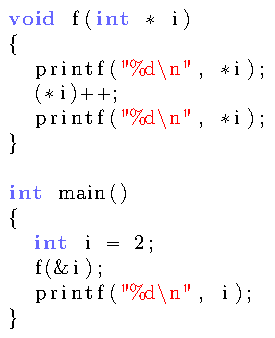
\includegraphics[width=4cm]{pics/sample-address.pdf}
};

\node at (7.5,3.5) {Pile};
\draw (6,-3) -- (6,3);
\draw (9,-3) -- (9,3);

%\foreach \i in {-2.5,-2,...,2.5}
%	\draw (6,\i) -- (9,\i);
\draw (6,-2.75) -- (9,-2.75);
\draw (6,2.75) -- (9,2.75);

\only<1->{\draw[white,->,>=stealth,ultra thick] (-2.8,-0.75) -- (-2.3,-0.75);} %phantom
\only<2>{\draw[comment-green,->,>=stealth,ultra thick] (-2.8,-0.75) -- (-2.3,-0.75);}
\only<3>{\draw[comment-green,->,>=stealth,ultra thick] (-2.8,-1.1) -- (-2.3,-1.1);}
\only<4>{\draw[comment-green,->,>=stealth,ultra thick] (-2.8,-1.4) -- (-2.3,-1.4);}
\only<5>{\draw[comment-green,->,>=stealth,ultra thick] (-2.8,2.18) -- (-2.3,2.18);}
\only<6>{\draw[comment-green,->,>=stealth,ultra thick] (-2.8,1.5) -- (-2.3,1.5);}
\only<7>{\draw[comment-green,->,>=stealth,ultra thick] (-2.8,1.1) -- (-2.3,1.1);}
\only<8>{\draw[comment-green,->,>=stealth,ultra thick] (-2.8,0.75) -- (-2.3,0.75);}
\only<9>{\draw[comment-green,->,>=stealth,ultra thick] (-2.8,0.4) -- (-2.3,0.4);}
\only<10>{\draw[comment-green,->,>=stealth,ultra thick] (-2.8,-1.8) -- (-2.3,-1.8);}

%\only<3->{\node at (5.25,-2.35) {\scriptsize \texttt{0xCAFE}};}
\only<3-6>{\filldraw[blue!60, fill=blue!60, rounded corners=2mm] (6.1,-2.65) rectangle (8.9,-2.05) node[midway,black] {$2$};}
\only<7->{\filldraw[blue!60, fill=blue!60, rounded corners=2mm] (6.1,-2.65) rectangle (8.9,-2.05) node[midway,black] {$3$};}
\only<3->{\node[anchor=east] at (5.5,-2.35) {\scriptsize 0xCAFE : \texttt{i}};}

\only<4-9>{\filldraw[blue!60, fill=blue!60, rounded corners=2mm] (6.1,-1.95) rectangle (8.9,-1.05) node[midway,black] {\texttt{0xCAFE}};}
\only<4-9>{\node[anchor=east] at (5.5,-1.35) {\scriptsize 0xCAF6 : \texttt{\&i}};}

\only<5-8>{\filldraw[blue!60, fill=blue!60, rounded corners=2mm] (6.1,0.7) rectangle (8.9,1.6) node[midway,black] {\texttt{0xCAFE}};}
%\only<7-8>{\filldraw[blue!60, fill=blue!60, rounded corners=2mm] (6.1,1) rectangle (8.9,1.6) node[midway,black] {$3$};}
\only<5-8>{\node[anchor=east] at (5.5,1.15) {\scriptsize Copie de \texttt{\&i}};}
\only<5-8>{\draw[thick,->,red!80] (5.95,1.15) to[out=240,in=120] (5.95,-2.35);}

\only<9->{\filldraw[blue!10, fill=blue!10, rounded corners=2mm] (6.1,0.7) rectangle (8.9,1.6) node[midway,black!30] {\texttt{0xCAFE}};}
\only<9->{\node[black!30,anchor=east] at (5.5,1.15) {\scriptsize Copie de \texttt{\&i}};}
\only<9->{\draw[thick,->,red!10] (5.95,1.15) to[out=240,in=120] (5.95,-2.35);}
\only<4-9>{\draw[thick,->,red!80] (5.95,-1.35) to[out=240,in=120] (5.95,-2.35);}

\only<10->{\filldraw[blue!10, fill=blue!10, rounded corners=2mm] (6.1,-1.95) rectangle (8.9,-1.05) node[midway,black!30] {\texttt{0xCAFE}};}
\only<10->{\node[anchor=east,black!30] at (5.5,-1.35) {\scriptsize 0xCAF6 : \texttt{\&i}};}
\only<10->{\draw[thick,->,red!10] (5.95,-1.35) to[out=240,in=120] (5.95,-2.35);}
\end{tikzpicture}
\end{center}
\end{frame}

\begin{frame}[containsverbatim]
\frametitle{Exemple}
\begin{itemize}[<+->]
\item Fichier \texttt{swap-addr-wrong.c}
\end{itemize}
\begin{lstlisting}
void swap(int * ptx, int * pty)
{
	printf("Entering swap : %d %d\n", *ptx, *pty);

	int* tmp = pty;
	pty = ptx;
	ptx = tmp;

	printf("Exiting swap : %d %d\n", *ptx, *pty);
}

int main()
{
	int x = 2;
	int y = 3;

	printf("Before call : %d %d\n", x, y);
    swap(&x, &y);
    printf("After call : %d %d\n", x, y);
}
\end{lstlisting}
\end{frame}

\begin{frame}[containsverbatim]
\frametitle{Exemple}
\begin{itemize}[<+->]
\item Fichier \texttt{swap-addr.c}
\end{itemize}
\begin{lstlisting}
void swap(int * ptx, int * pty)
{
	printf("Entering swap : %d %d\n", *ptx, *pty);

	int tmp = *pty;
	*pty = *ptx;
	*ptx = tmp;

	printf("Exiting swap : %d %d\n", *ptx, *pty);
}

int main()
{
	int x = 2;
	int y = 3;

	printf("Before call : %d %d\n", x, y);
    swap(&x, &y);
    printf("After call : %d %d\n", x, y);
}
\end{lstlisting}
\end{frame}

\begin{frame}
\frametitle{Retour d'une fonction}
\begin{itemize}[<+->]
\item Comme pour le passage de paramètre, le retour d'une fonction peut être effectué
	\begin{itemize}
	\item par valeur (par défaut) : \lstinline|int f();|
	\item par adresse : \lstinline|int* f();|
	\end{itemize}
\end{itemize}
\begin{alertblock}<+->{Attention}
	\begin{itemize}[<+->]
	\item Ne créez pas de pointeurs vers des temporaires
	\item Ils vont « pendouiller » (dangling)
	\end{itemize}
\end{alertblock}
\end{frame}

\begin{frame}[containsverbatim]
\frametitle{Illustration}
\begin{itemize}
\item Fichier \texttt{return.c}
\end{itemize}
\begin{lstlisting}
int f() //ok
{
    int i = 42;
    return i;
}

int* g() //wrong
{
    int i = 42;
    int * pti = &i;
    return pti;
}

void h(int * pt)  //wrong
{
    int i = 42;
    pt = &i;
}

void hh(int * pt) //also wrong
{
    int i = 42;
    *pt = i;
}
\end{lstlisting}
\end{frame}

\section{Fonctions inline}

\begin{frame}
\frametitle{Fonctions inline}
\begin{itemize}[<+->]
\item Fonction dont le corps est substitué à l'appel
\end{itemize}
\begin{exampleblock}<+->{Avantages}
	\begin{itemize}[<+->]
	\item Gain de temps (pas de \texttt{call})
	\end{itemize}
\end{exampleblock}
\begin{alertblock}<+->{Inconvénients}
	\begin{itemize}[<+->]
	\item Exécutable grossit (copier / coller)
	\end{itemize}
\end{alertblock}
\begin{itemize}[<+->]
\item Non contraignant : « demande courtoise »
\item Ces fonctions n'ont \emph{pas} d'adresse
\item Déclarée avec le mot-clé \lstinline|inline|
\end{itemize}
\end{frame}

\begin{frame}[containsverbatim]
\frametitle{Exemple}
\begin{itemize}
\item Fichier \texttt{inline.c}
\end{itemize}
\begin{lstlisting}
void for_each(int* array, unsigned n, int (*f)(int))
{
    for(unsigned i = 0; i < n; i++)
        array[i] = f(array[i]);
}

int plus_one(int i)
{
    return i + 1;   
}

inline int plus_two(int i)
{
    return i + 2;   
}

int main()
{
    int array[] = {1,2,3,4,5};
    for_each(array, 5, plus_one);
    for(unsigned i = 0; i < 5; i++)
        printf("%d ", array[i]);
    printf("\n");
     
    for_each(array, 5, plus_two); //wrong
}
\end{lstlisting}
\end{frame}

\end{document}
